\iffalse
\let\negmedspace\undefined
\let\negthickspace\undefined
\documentclass[journal,12pt,onecolumn]{IEEEtran}
\usepackage{cite}
\usepackage{amsmath,amssymb,amsfonts,amsthm}
\usepackage{algorithmic}
\usepackage{graphicx}
\usepackage{textcomp}
\usepackage{xcolor}
\usepackage{txfonts}
\usepackage{listings}
\usepackage{enumitem}
\usepackage{circuitikz}
\usepackage{mathtools}
\usepackage{gensymb}
\usepackage{comment}
\usepackage[breaklinks=true]{hyperref}
\usepackage{tkz-euclide} 
\usepackage{listings}
\usepackage{gvv}    
\usepackage{enumitem}
\usepackage{amsmath}
\def\inputGnumericTable{}                                 
\usepackage[latin1]{inputenc}                                
\usepackage{color}                                            
\usepackage{array}                                            
\usepackage{longtable}                                       
\usepackage{calc}                                             
\usepackage{multirow}                                         
\usepackage{hhline}                                           
\usepackage{ifthen}                                           
\usepackage{lscape}
\usepackage{tabularx}

\newtheorem{theorem}{Theorem}[section]
\newtheorem{problem}{Problem}
\newtheorem{proposition}{Proposition}[section]
\newtheorem{lemma}{Lemma}[section]
\newtheorem{corollary}[theorem]{Corollary}
\newtheorem{example}{Example}[section]
\newtheorem{definition}[problem]{Definition}
\newcommand{\BEQA}{\begin{eqnarray}}
\newcommand{\EEQA}{\end{eqnarray}}
\newcommand{\define}{\stackrel{\triangle}{=}}
\theoremstyle{remark}
\newtheorem{rem}{Remark}
\begin{document}
\bibliographystyle{IEEEtran}
\vspace{3cm}

\title{GATE:2022 - BM 54 }
\author{EE23BTECH11025 - Anantha Krishnan $^{}$% <-this % stops a space
}
\maketitle
\bigskip



\section{question}

A series RLC circuit is connected to 220 V, 50 Hz supply. For a fixed a value of R and C, the inductor L is varied to deliver the maximum current. This value 0.4A and the corresponding potential drop across the capacitor is 330 V. The value of the inductor L is ? (Rounded off to two decimal places).
 



\textbf{Solutions :}
\fi




\begin{table}[ht!]
\centering
\begin{tabular}{ |c|c|c| } 
 \hline
Symbols & Description & Values  \\
\hline
 $V_s$ & Input voltage & 220 V and 50Hz\\
 \hline
 $\chi_L$ & Impedance across inductor & $j\omega L$\\
 \hline
 $\chi_C$ & Impedance across capacitor & $\frac{-j}{\omega C}$\\
 \hline
 $Z$& Impedance across the entire circuit & $\frac{1}{R+j\omega L +\frac{-j}{\omega C}}$\\
 \hline
\end{tabular}
\caption{Parameters, Descriptions, and Values}
\label{table:ee25-bm54-gate2022}
\end{table}






    
    \ctikzset{bipoles/thickness=1.2}
    \newcommand{\midlabelline}[3]{
   \node (midlabel) at ($ (#1)!.5!(#2) $) {#3};
   \draw[latex-] (#1) --  (midlabel);
   \draw[-latex] (midlabel) -- (#2);
}

\begin{enumerate}
\begin{center}
\begin{circuitikz}[scale=0.8]
    % Circuit
    \draw[line width=0.6]
        (1.5,5) to [sinusoidal voltage source, l_=$220V$${,}50Hz$, i=$I$] (1.5,1)
        (1.5,5) to [resistor, l_=$R$] ++(4,0) to [inductor, l_=$L$] ++(0,-4) to [capacitor, l_=$C$] +(-4,0) ;
    
    % Voltage Infos
    \midlabelline{1.5,5.5}{5.5,5.5}{$V(R)$}
    \midlabelline{6.5,5}{6.5,1}{$V(L)$}
    \midlabelline{1.5,0}{5.5,0}{$V(C)$}
    
    % Grid
    %\draw[help lines] (0,0) grid (7,6);
\end{circuitikz}
\end{center}
    \end{enumerate}
During maximum current$\quad\abs{Z}$ is minimum .
\begin{align}
I &= \frac{V_s}{Z}\\
 &= \frac{V_s}{R+\chi_{L}+\chi_{C}}\\ 
 &=\frac{V_s}{R+j\omega L+\frac{1}{j\omega C}}\label{eq:ee25-gate2-1}\\
\quad \abs{I}&={\frac{\quad \abs{V_s}}{\sqrt{R+\brak{\omega L-\frac{1}{\omega C}^2}}}}
\end{align}
Varying $L$ for maximum value of ${I}$ :
\begin{align}
\omega L = \frac{1}{\omega C} \label{eq:ee25-gate2-2}
\end{align}
Putting in $\eqref{eq:ee25-gate2-1}$:
\begin{align}
    I_{max} &= \frac{V_s}{R}
\end{align}
$I_{max}$ has same phase as $V_s$ (Assume $\angle{\phi})$.
For impedance across the capacitor :
\begin{align}
 \left.V_C\right|_{I=I_{max}}&= I_{max} \chi_C\\
-330\angle{\brak{90+\phi}} &= \brak{0.4\angle{\phi}}\chi_C\\
-330\angle{90} &= 0.4\chi_C\\
\implies \chi_C &= -825j\si{\ohm}
\end{align}
For value of Capacitor and inductor, using \eqref{eq:ee25-gate2-2} :
\begin{align}
L &= \frac{825}{100\pi}H\\
&\approx 2.63 \si{H}\\
C &= 3.858*10^{-6} \si{F}
\end{align}


    \begin{figure}[!ht]    
    \centering
\graphicspath{ {2022/BM/54/figs/} }
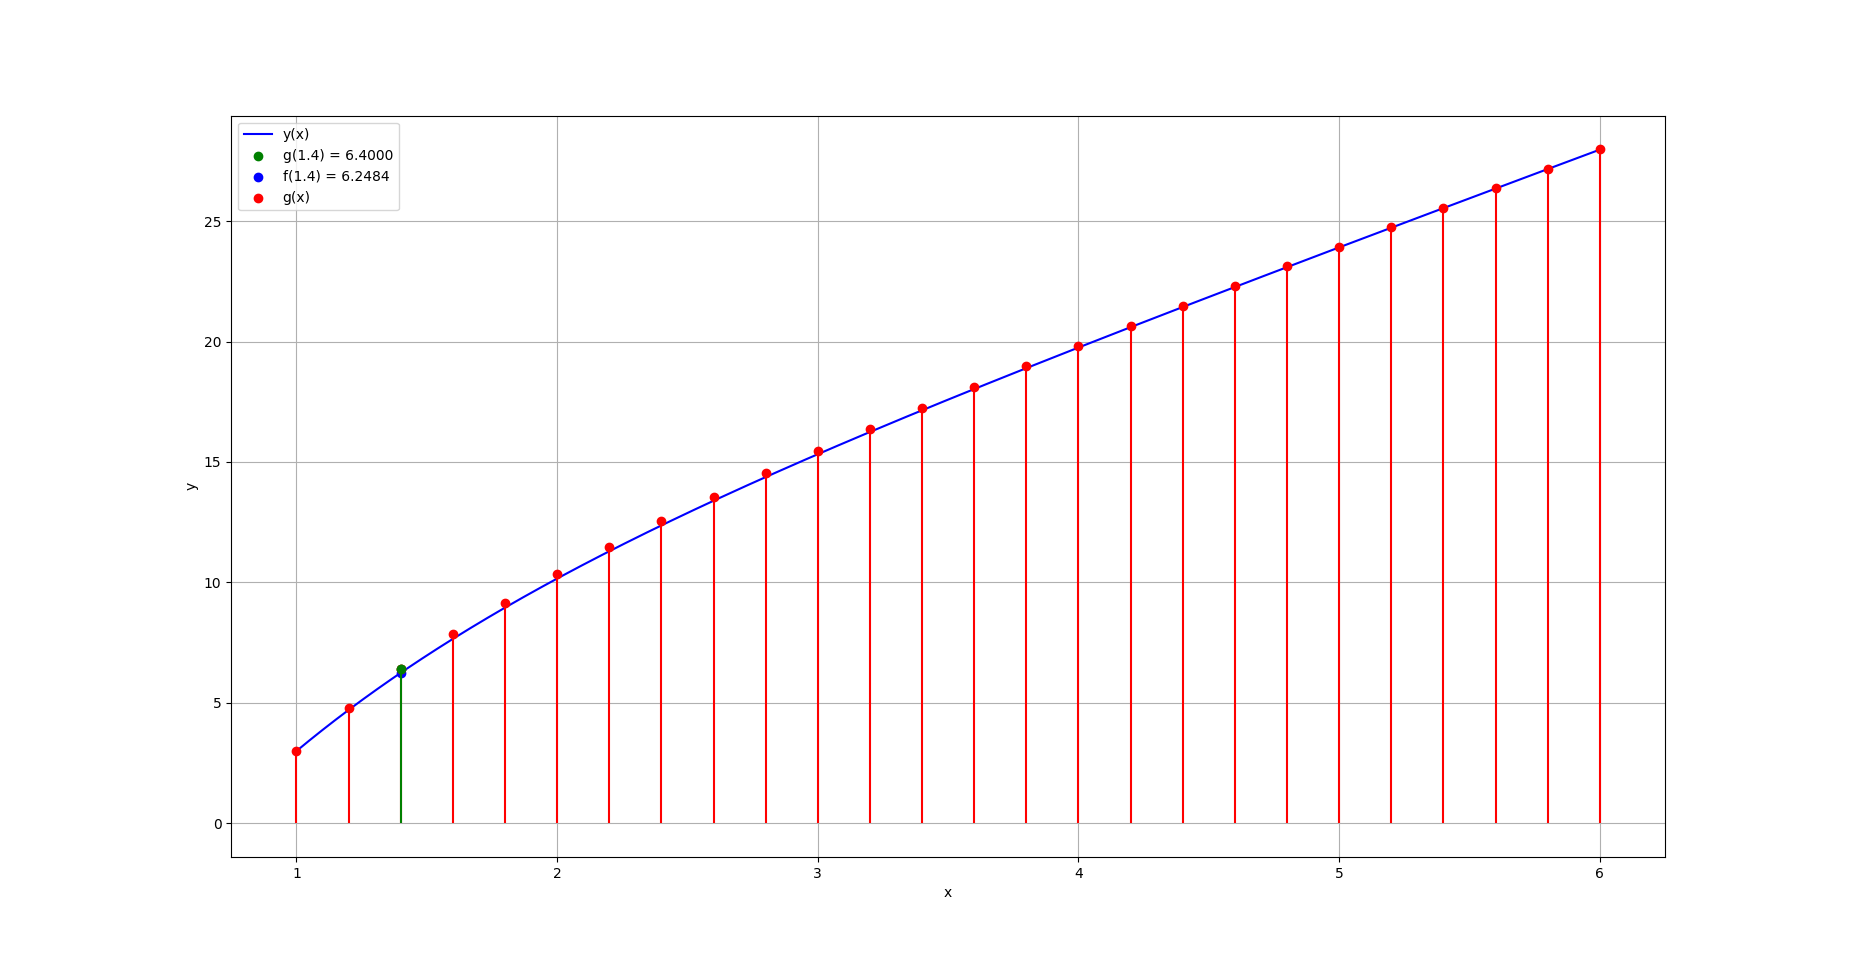
\includegraphics[width=\columnwidth]{graph_1}
\caption{ $I$ vs $L$ }
\label{graph:ee25-gate2-graph}
\end{figure}







